%% ----------------------------------------------------------------
%% Thesis.tex -- main
%% ---------------------------------------------------------------- 

\documentclass[a4paper, 10pt, oneside]{memoir}
%% Use the option citeauthor to be able to use citet. The default cite will still work.
\usepackage[citeauthor]{basilea}

%% ----------------------------------------------------------------

\title				{Optimizing Symbolic Execution Through Taint Analysis and Path Prioritization}
\thesistype			{Bachelor thesis}

\department 		{Department of Mathematics and Computer Science}
\faculty			{Natural Science Faculty of the University of Basel}
\research		    {Databases and Information Systems (DBIS) Group \\ \url{https://dbis.dmi.unibas.ch/}}

\examiner    		{Dr. Marco Vogt}
\supervisor  		{Prof. Dr. Christopher Scherb}

\authors     		{Ruben Hutter}
\email				{ruben.hutter@unibas.ch}
\immatriculnr		{2020-065-934}

\date				{02.07.2025}

% switch here for the german logo to logo-de
\ulogo				{Template/logo-en} 


%% ----------------------------------------------------------------
\begin{document}

% for english use \selectlanguage{english}, for german use \selectlanguage{ngerman}
\selectlanguage{english}

\thesisfront
\maketitle
\pagestyle{thesis}
%% ----------------------------------------------------------------
% !TEX root = ../Thesis.tex
\chapter{Acknowledgments}

I would like to express my sincere gratitude to Prof. Dr. Christopher Scherb for his supervision and guidance throughout this thesis. His expertise in program analysis and symbolic execution provided essential direction for this research.

I am grateful to Dr. Marco Vogt for his role as examiner and for facilitating the opportunity to pursue this research topic. His feedback and suggestions helped refine both the technical approach and the presentation of this thesis.

I would like to thank Ivan Giangreco for providing the LaTeX thesis template used for this document, which greatly facilitated its formatting and structure.

I also acknowledge my fellow student Nico Bachmann for developing the Schnauzer visualization library, which enhanced the presentation and analysis of the results.

I thank my family and friends for their encouragement and support during my studies, which made completing this thesis possible.

Finally, I acknowledge the developers of the angr binary analysis framework, whose comprehensive platform enabled the implementation of the techniques described herein.

%% ----------------------------------------------------------------
% !TEX root = ../Thesis.tex
\chapter{Abstract}

Symbolic execution is a powerful program analysis technique widely used for vulnerability discovery and test case generation. However, its practical application is often hampered by scalability issues, primarily due to the "path explosion problem" where the number of possible execution paths grows exponentially with program complexity. This thesis addresses this fundamental challenge by proposing an optimized approach to symbolic execution that integrates taint analysis and path prioritization.

The core contribution is a novel exploration strategy that moves away from uniform path exploration towards targeted analysis of security-critical program behaviors. The approach prioritizes execution paths originating from memory allocations and user input processing points, as these represent common sources of vulnerabilities. By leveraging dynamic taint analysis, the system identifies and tracks data flow from these critical sources, enabling the symbolic execution engine to focus computational resources on paths influenced by tainted data while deprioritizing paths with no dependency on external inputs.

% TODO: Benchmark to test if this is actually true
The implementation integrates this taint-guided exploration strategy with the angr symbolic execution framework, introducing a scoring mechanism that dynamically adjusts path prioritization based on taint propagation. The effectiveness of this optimization is evaluated through comparative analysis, examining runtime efficiency, path coverage quality, and vulnerability discovery capabilities. Results demonstrate that this approach can significantly reduce the search space while maintaining or improving the detection of security-relevant program behaviors, making symbolic execution more practical for large and complex software systems.

%% ----------------------------------------------------------------
\thesistoc
%% ----------------------------------------------------------------
%\thesisnomencl
%% ----------------------------------------------------------------
\thesismain
% !TEX root = ../Thesis.tex
\chapter{Introduction}

Symbolic execution has emerged as one of the most powerful techniques for automated program analysis, offering significant advantages over traditional testing methods for vulnerability discovery and test case generation. By representing program inputs as symbolic variables rather than concrete values, symbolic execution engines can systematically explore multiple execution paths within a single analysis run, potentially uncovering bugs that would be difficult to find through conventional testing approaches.

Despite its theoretical promise, symbolic execution faces a fundamental scalability challenge known as the ``path explosion problem.'' As program complexity increases, the number of possible execution paths grows exponentially, quickly overwhelming computational resources and rendering the analysis intractable for real-world software systems. This limitation has been a persistent barrier to the widespread adoption of symbolic execution in practical security analysis workflows.

Current symbolic execution engines typically employ uniform exploration strategies, treating all program paths with equal priority regardless of their potential security relevance. This approach wastes significant computational resources on code paths that are unlikely to contain vulnerabilities, while potentially missing critical security-sensitive execution flows. For instance, paths that process user-controlled input or handle memory allocations are statistically more likely to contain exploitable vulnerabilities than paths that perform simple arithmetic operations or access read-only data structures.

This thesis addresses the path explosion problem by proposing a novel approach that integrates taint analysis with symbolic execution to enable intelligent path prioritization. The core insight is that not all execution paths are equally important from a security perspective. By leveraging taint analysis to identify and track data flow from critical sources such as user inputs and memory allocation sites, we can guide the symbolic execution engine to focus its computational resources on paths most likely to exhibit security-relevant behaviors.

The proposed approach introduces a dynamic scoring mechanism that continuously evaluates the security relevance of execution states based on taint propagation patterns. States that process tainted data receive higher priority scores, while states operating exclusively on untainted data are deprioritized or pruned entirely. This selective exploration strategy aims to maintain the thoroughness of symbolic execution for security-critical code while dramatically reducing the analysis time by avoiding exhaustive exploration of irrelevant program regions.

The main contributions of this work are:

\textbf{Taint-Guided Path Prioritization:} A novel integration of dynamic taint analysis with symbolic execution that uses taint propagation patterns to intelligently prioritize exploration of security-relevant execution paths.

\textbf{Adaptive Scoring Algorithm:} A scoring mechanism that dynamically adjusts path priorities based on real-time taint analysis results, enabling the symbolic execution engine to focus computational resources on the most promising program regions.

\textbf{Practical Implementation:} A complete implementation of the proposed approach using the angr symbolic execution framework, demonstrating the feasibility and effectiveness of taint-guided exploration in a production-quality tool.

\textbf{Empirical Evaluation:} Comprehensive evaluation comparing the proposed approach against standard symbolic execution techniques, measuring improvements in analysis efficiency, vulnerability discovery rate, and overall scalability.

The effectiveness of this optimization is evaluated through extensive experimentation on representative programs, examining key metrics including runtime efficiency, path coverage quality, and vulnerability detection capabilities. Results demonstrate that the taint-guided approach can significantly reduce analysis time while maintaining or improving the detection of security-relevant program behaviors, making symbolic execution more practical for analyzing large and complex software systems.

The remainder of this thesis is organized as follows. Chapter 2 provides essential background on symbolic execution, taint analysis, and the angr framework that forms the foundation for this work. Chapter 3 presents the conceptual framework and theoretical algorithms underlying the taint-guided exploration strategy. Chapter 4 details the practical implementation, including integration with angr and the design of the scoring mechanism. Chapter 5 presents a comprehensive evaluation of the approach, comparing its performance against standard symbolic execution techniques. Chapter 6 discusses related work in symbolic execution optimization and path prioritization. Chapter 7 concludes with a summary of contributions and implications for future research. Chapter 8 explores potential extensions and future research directions, while Chapter 9 documents the use of AI-assisted technologies in the development of this thesis.

% !TEX root = ../Thesis.tex
\chapter{Background}

This chapter establishes the theoretical foundations necessary for understanding the taint-guided symbolic execution optimization presented in this thesis. We examine symbolic execution, taint analysis, control flow analysis, and the Angr framework.

\section{Symbolic Execution}

Symbolic execution is a program analysis technique that explores execution paths by using symbolic variables instead of concrete inputs. The program state consists of symbolic variables, path constraints, and a program counter. When execution encounters a conditional branch, the engine explores both branches by adding appropriate constraints to the path condition.

A fundamental challenge in symbolic execution is the path explosion problem. As program complexity increases, the number of possible execution paths grows exponentially, making exhaustive exploration computationally intractable. This scalability issue particularly affects real-world applications with complex control flow structures and deep function call hierarchies. Research has shown that symbolic execution tools designed to optimize statement coverage often fail to cover potentially vulnerable code due to complex system interactions and scalability issues of constraint solvers \cite{schwartz_all_2010}.

Traditional symbolic execution typically employs a forward approach, starting from the program's entry point and exploring paths toward potential targets. However, this method may struggle to reach deeply nested functions or specific program locations of interest. Backward symbolic execution, conversely, begins from target locations and works backwards to identify input conditions that can reach those targets. Compositional approaches combine both techniques by analyzing individual functions in isolation and then reasoning about their interactions.

The scalability challenges of symbolic execution have motivated numerous optimization approaches, including state merging, constraint optimization, and path prioritization strategies. These optimization techniques form the foundation for more targeted analysis approaches that focus computational resources on security-relevant program behaviors.

\section{Taint Analysis}

Taint analysis tracks the propagation of data derived from untrusted sources throughout program execution. Data originating from designated sources (such as user input functions like \texttt{fgets}, \texttt{gets}, \texttt{read}, or \texttt{scanf}) is marked as ``tainted.'' The analysis tracks how this tainted data flows through assignments, function calls, and other operations. When tainted data reaches a security-sensitive sink (such as buffer operations or system calls), the analysis flags a potential vulnerability.

The propagation rules define how taint spreads through different operations: assignments involving tainted values result in tainted variables, arithmetic operations with tainted operands typically produce tainted results, and function calls with tainted arguments may result in tainted return values depending on the function's semantics. Dynamic taint analysis performs tracking during program execution, providing precise information about actual data flows while considering specific calling contexts and program states, resulting in reduced false positives compared to static analysis approaches.

The combination of taint analysis and symbolic execution creates a powerful analysis framework. Symbolic execution can explore multiple program paths while taint analysis identifies which paths involve security-relevant data flows. Research has demonstrated effective integration through pipelined approaches that achieve significant performance improvements while maintaining precision \cite{ming_taintpipe_2015}. This integration enables targeted exploration of paths that process untrusted input, significantly improving the efficiency of vulnerability discovery \cite{newsome_dynamic_2005}.

\section{Control Flow Analysis}

Control flow analysis examines the possible execution paths through a program by constructing and analyzing control flow graphs (CFGs). A CFG represents program structure where nodes correspond to basic blocks of sequential instructions and edges represent possible control transfers between blocks. This representation enables systematic analysis of program behavior and reachability properties.

Static analysis constructs CFGs by examining program code without executing it, analyzing structure and control flow based solely on the source code or binary representation. This approach offers comprehensive coverage and efficiency, enabling examination of all statically determinable program paths without requiring specific input values. However, static analysis faces limitations including difficulty with indirect call resolution and potential false positives due to conservative approximations required for soundness.

Dynamic analysis executes the program and collects runtime information, providing precise information about actual program behavior and complete execution context. This approach eliminates many false positives inherent in static analysis and validates that control flow relationships are actually exercised under realistic conditions. However, dynamic analysis results depend heavily on input quality and coverage.

A Call Graph represents function call relationships within a program, where each node corresponds to a function and each directed edge represents a call relationship. Call graphs serve important purposes including program understanding, entry point identification, reachability analysis, and complexity assessment. Call graphs prove valuable for path prioritization strategies, enabling identification of functions reachable from tainted input sources and assessment of their relative importance in program execution flow.

Modern analysis tools often combine both static and dynamic approaches. Hybrid techniques leverage the efficiency of static analysis for initial program understanding while using dynamic analysis to resolve ambiguities and validate findings under realistic execution conditions.

\section{Angr Framework}

Angr is an open-source binary analysis platform providing comprehensive capabilities for static and dynamic program analysis \cite{shoshitaishvili_sok_2016}. The platform supports multiple architectures and provides a Python-based interface for research and education \cite{springer_teaching_2018}. Key components include the Project object representing the binary under analysis with access to contents, symbols, and analysis capabilities; the Knowledge Base storing information gathered during analysis including function definitions and control flow graphs; the Simulation Manager handling multiple program states during symbolic execution and managing state transitions; and the Solver Engine interfacing with constraint solvers to determine path feasibility and solve for concrete input values.

Angr supports both static (\texttt{CFGFast}) and dynamic (\texttt{CFGEmulated}) CFG construction. Static analysis provides efficiency but may miss indirect calls, while dynamic analysis offers completeness at higher computational cost \cite{angr_documentation}. The static approach analyzes the binary without execution, making it efficient for initial program understanding, while dynamic analysis executes the program with sample inputs to discover reachable code, providing more complete coverage of actual execution paths and better handling of indirect calls.

Angr represents program states with register values, memory contents, path constraints, and execution history. The framework provides APIs for state inspection and manipulation, along with fine-grained execution control through step functions and exploration techniques. The step function advances execution by single instructions, enabling precise control over exploration processes, while various exploration strategies guide path selection including depth-first search, breadth-first search, and custom heuristics. Configuration options control execution behavior, such as handling of unconstrained memory and registers, allowing researchers to customize analysis behavior for specific research requirements.

The framework's extensible architecture enables integration of custom analysis techniques, making it particularly suitable for implementing novel symbolic execution optimizations. Angr's support for both static and dynamic analysis capabilities provides the foundation necessary for implementing taint-guided exploration strategies that combine control flow analysis with symbolic execution.

Multiple symbolic execution frameworks have been developed to address the scalability challenges discussed earlier \cite{baldoni_survey_2018}. While angr focuses on binary analysis and provides a comprehensive platform for security research, other frameworks target different domains and approaches. KLEE \cite{cadar_klee_2008} remains one of the most prominent tools for C programs, focusing on automatic test generation and providing extensive coverage analysis capabilities. SAGE \cite{godefroid_automated_2008} extends symbolic execution to binary code analysis through whitebox fuzzing, particularly effective for vulnerability discovery in Windows applications. CBMC \cite{clarke_behavioral_2003} offers bounded model checking for C/C++ programs with formal verification capabilities. Java PathFinder \cite{visser_model_2003} provides symbolic execution for Java bytecode with emphasis on model checking applications. Each framework offers distinct advantages: KLEE excels in systematic path exploration for source code, SAGE in practical vulnerability discovery for binaries, CBMC in formal verification, and Java PathFinder in model checking for Java applications.

% !TEX root = ../Thesis.tex
\chapter{Improving Symbolic Execution ...}

This is a short conclusion on the thesis template documentation. If you have any comments or suggestions for improving the template, if you find any bugs or problems, please contact me. 

How does it work conceptually? (not implementation) which path i choose and why. limiter -> je weiter unter desto schwieriger dass ich eine vulnerability triggere
Pseudo code of the algorithm


% !TEX root = ../Thesis.tex
\chapter{Practical Implementation}

This is a short conclusion on the thesis template documentation. If you have any comments or suggestions for improving the template, if you find any bugs or problems, please contact me. 

How does the script work? Implementation details, how to use it, how to run it, how to set up the environment. Strategies that I use, LoopSeer...


% !TEX root = ../Thesis.tex
\chapter{Evaluation}

%Compare my work to default angr strategy. Implement a benchmark tool to compare the performance of the taint-guided symbolic execution against the default path exploration strategy in angr. The benchmark should include:
%\begin{itemize}
%    \item A set of test programs with known vulnerabilities.
%    \item Metrics for evaluation:
%    \begin{itemize}
%        \item Execution time
%        \item Number of paths explored
%        \item Vulnerabilities detected
%        \item Path coverage
%    \end{itemize}
%    \item Comparison of results between the taint-guided approach and the default angr strategy.
%\end{itemize}

\section{Experimental Design}
\subsection{Research Questions}
\begin{enumerate}
    \item How does taint-guided exploration compare to default symbolic execution in terms of vulnerability discovery rate?
    \item What is the computational overhead of taint tracking and scoring?
    \item How does the approach scale with program complexity?
    \item What is the effectiveness of different taint source configurations?
\end{enumerate}

\subsection{Evaluation Metrics}
\begin{itemize}
    \item \textbf{Coverage Metrics:} Basic block coverage, path coverage
    \item \textbf{Efficiency Metrics:} Time to first vulnerability, total analysis time
    \item \textbf{Effectiveness Metrics:} Number of vulnerabilities found, false positive rate
    \item \textbf{Scalability Metrics:} Memory usage, state explosion control
\end{itemize}

\section{Benchmark Programs}
\subsection{Synthetic Benchmarks}
% Simple C programs with known vulnerabilities
% Buffer overflows, format string bugs, use-after-free

\subsection{Real-World Programs}
% DARPA CGC binaries
% CVE-documented vulnerable programs
% Open-source utilities with known security issues

\section{Experimental Results}
\subsection{Comparison with Standard Symbolic Execution}
% Tables and graphs comparing TraceGuard vs. default Angr
% Statistical significance testing

\subsection{Ablation Studies}
% Impact of different scoring components
% Effect of depth limitations
% Sensitivity to configuration parameters

\section{Case Studies}
\subsection{Buffer Overflow Discovery}
% Detailed trace of how TraceGuard finds a specific vulnerability
% Comparison with manual analysis

\subsection{Format String Vulnerability}
% Another detailed case study
% Demonstration of taint flow from input to vulnerable sink

% !TEX root = ../Thesis.tex
\chapter{Conclusion}

Rückblick auf die Arbeit, was wurde erreicht (evtl. merge with Future Work)

% !TEX root = ../Thesis.tex
\chapter{Future Work}
This is a short conclusion on the thesis template documentation. If you have any comments or suggestions for improving the template, if you find any bugs or problems, please contact me. 

\vspace{2cm}

Good luck with your thesis!

% !TEX root = ../Thesis.tex
\chapter{Related Work}

Evtl. already mentioned in background chapter

Paper: Macke TO München

% !TEX root = ../Thesis.tex
\chapter{Usage of AI}
This is a short conclusion on the thesis template documentation. If you have any comments or suggestions for improving the template, if you find any bugs or problems, please contact me. 

\vspace{2cm}

Good luck with your thesis!

%% ----------------------------------------------------------------
\thesisappendix
\thesisbib
\begin{appendices}
	% !TEX root = ../Thesis.tex
\chapter{Appendix}

\section{State Explosion Test Program Source Code}

\begin{lstlisting}[language=C, label={lst:state_explosion_test_program}]
#include <stdio.h>
#include <string.h>

void create_many_string_states(char *input) {
    // Create branching based on string content (tainted)
    if (strlen(input) > 10) {
        printf("Long input\n");
    } else {
        printf("Short input\n");
    }

    if (input[0] == 'A') {
        printf("Starts with A\n");
    } else if (input[0] == 'B') {
        printf("Starts with B\n");
    } else {
        printf("Starts with other\n");
    }
}

void untainted_integer_branching() {
    int static_val = 25;  // Hardcoded, not tainted

    // Classical angr will explore these, TraceGuard should skip
    if (static_val > 20) {
        printf("Static val > 20\n");
    }
    if (static_val % 5 == 0) {
        printf("Static val divisible by 5\n");
    }
    if (static_val < 30) {
        printf("Static val < 30\n");
    }
}

void critical_vulnerability(char *dangerous_input) {
    char tiny_buffer[6];  // Extremely small
    strcpy(tiny_buffer, dangerous_input);  // Obvious overflow
    printf("Critical: %s\n", tiny_buffer);
}

int main() {
    char user_input[400];

    // Untainted branching - TraceGuard should skip
    untainted_integer_branching();

    printf("Enter string input: ");
    if (fgets(user_input, sizeof(user_input), stdin)) {
        // Remove newline
        user_input[strcspn(user_input, "\n")] = 0;

        // This creates tainted string-based branching
        create_many_string_states(user_input);

        // Clear vulnerability with tainted data
        critical_vulnerability(user_input);
    }
    return 0;
}
\end{lstlisting}
 
\end{appendices}
%% ----------------------------------------------------------------
\thesisback
\iflanguage{english}
  {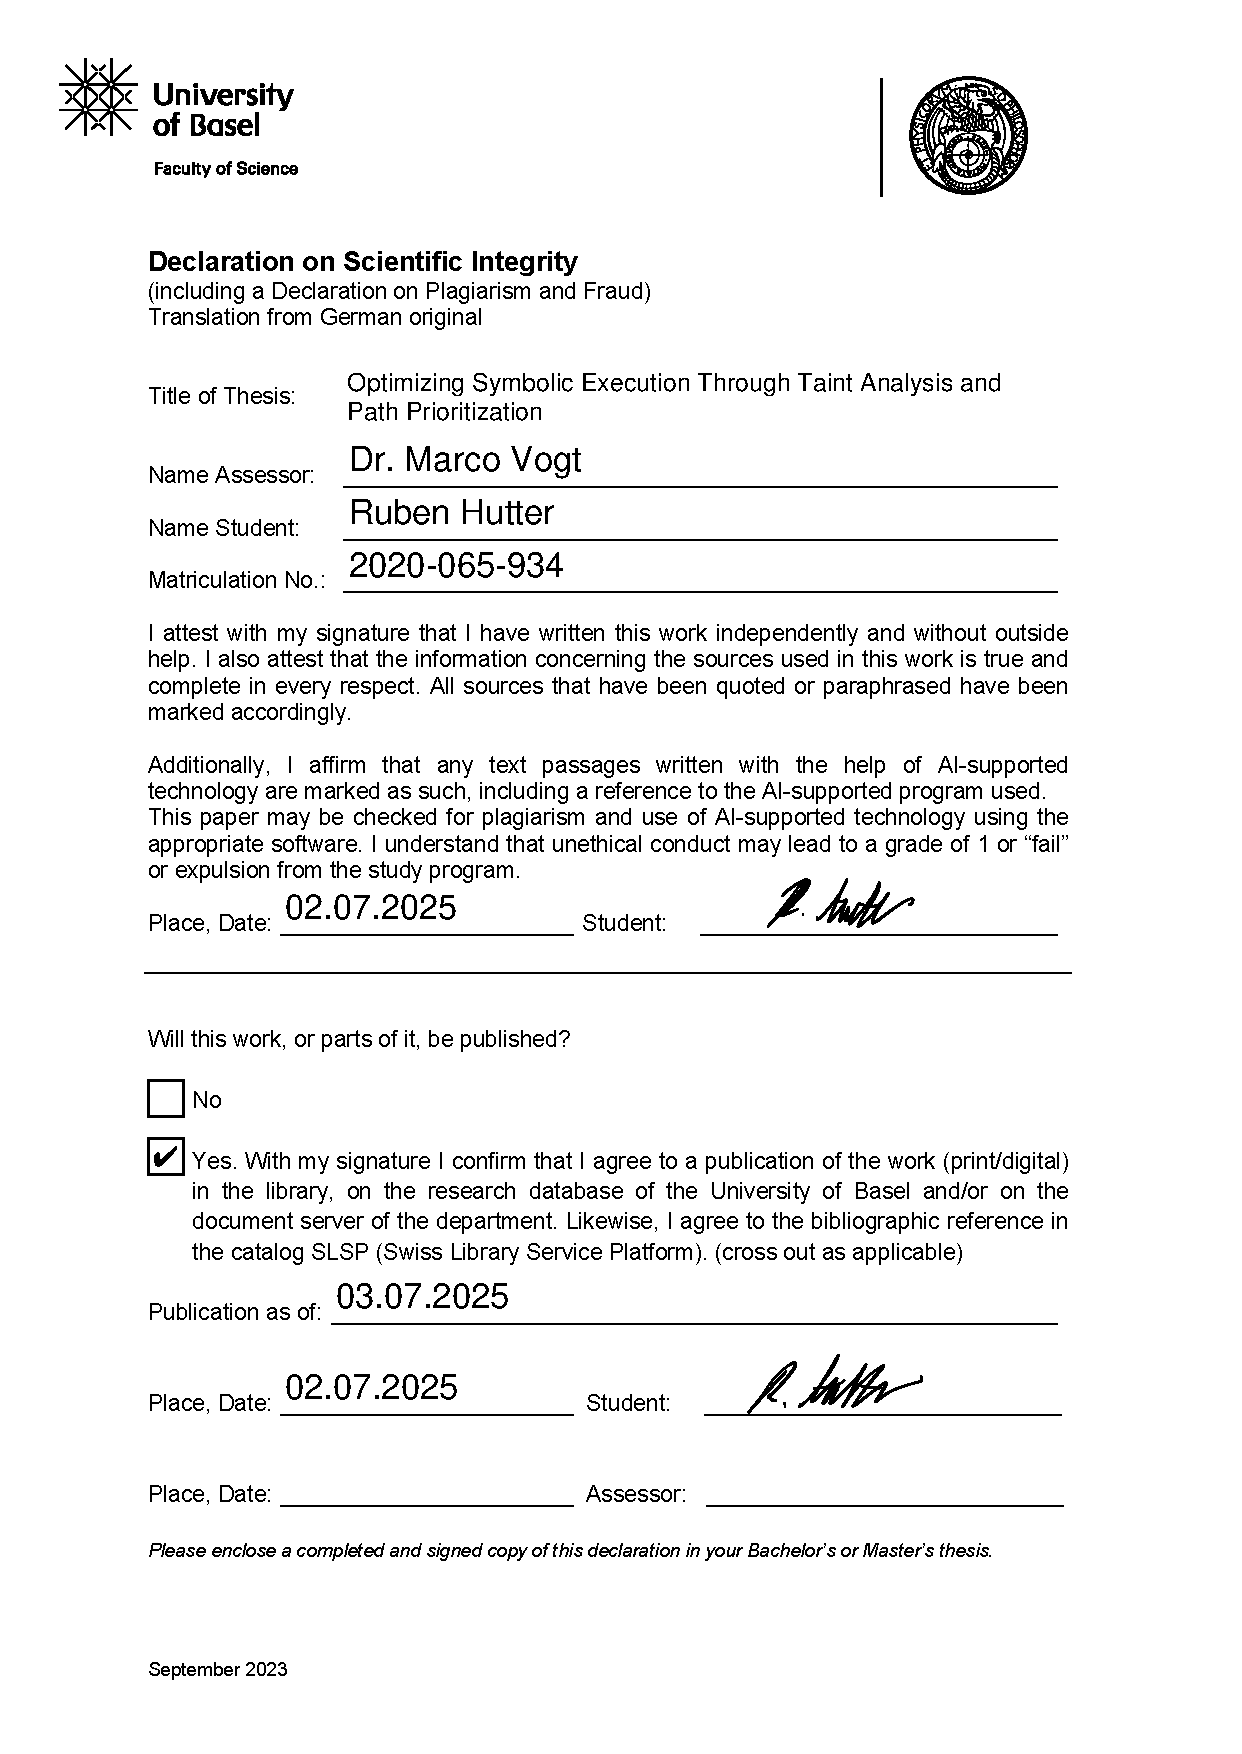
\includepdf{./Back/wissensch_Redlichkeit_E_09-2023.pdf}}
  {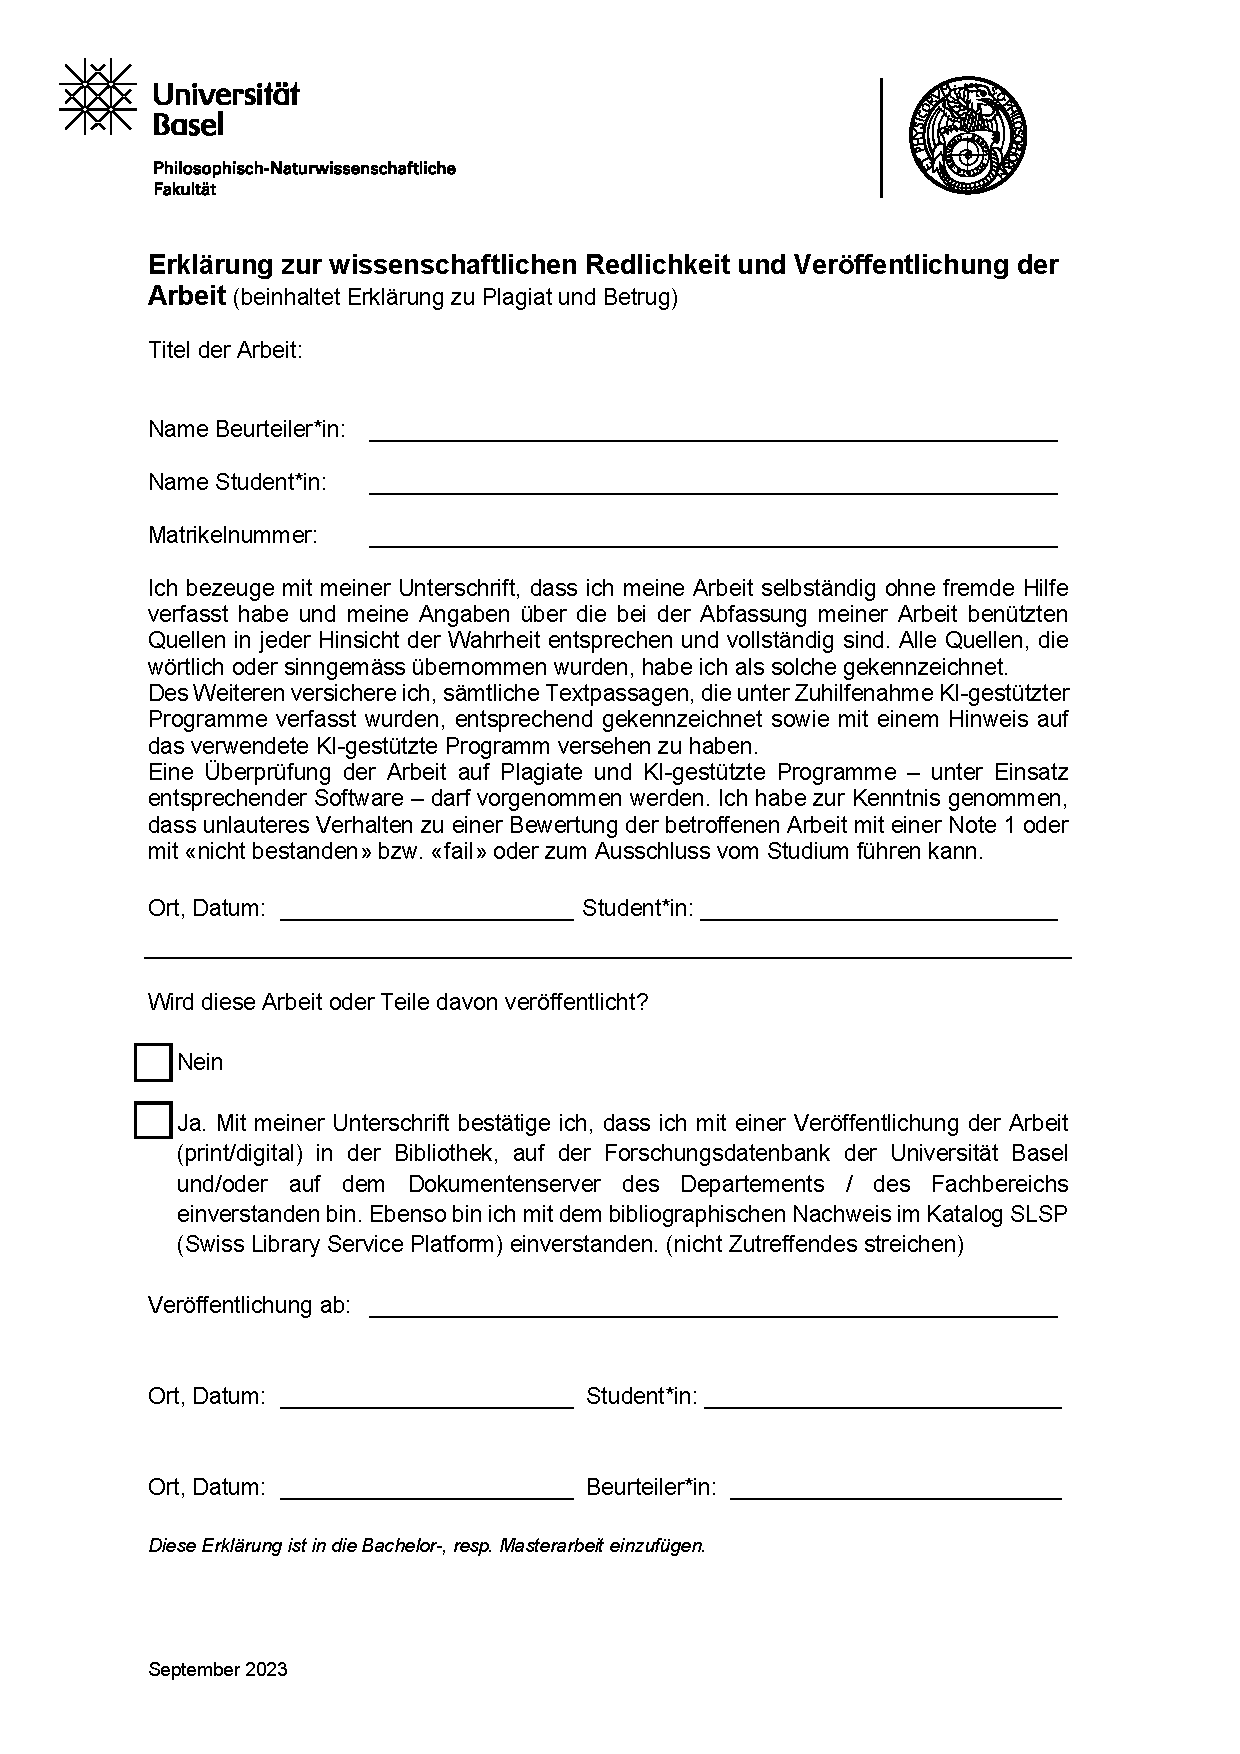
\includepdf{./Back/wissensch_Redlichkeit_D_09-2023.pdf}}
%% ----------------------------------------------------------------
\end{document}
%% ----------------------------------------------------------------
